

\section{Introduction}

%Motivate Prob KBs
%Describe Motivation of the the KHop system.
%Give example scenario.
%Introduce the Khop system.
%Describe intro that this demo show real time incremental changes and probability changes to a large KB.

In recent years, the large increase of machine accessible data has led researchers
to develop sophisticated methods of organizing and using the information.
In particular, the advance of information extraction techniques has allowed
millions of facts to be extracted from the web.
This is evidenced by the renewed interests in knowledge graphs and knowledge bases
from companies and
researchers~\cite{bellare2013woo,chang2014typed,dong2014knowledge,niu2012deepdive}.

Knowledge graphs efficiently store and manage the linking of facts.
Knowledge bases are equivalent to knowledge graphs but with an additional
inference engine. 
Inference engines allow the discovery of facts that are not explicitly
mentioned in the knowledge graph.
Researchers currently pair probabilities with extracted facts and rules to
represent the natural uncertainty found in language and extraction systems.
These systems are called probabilistic knowledge bases~\cite{chen2014knowledge}.
When performing inference, probabilistic knowledge bases consider the uncertainty
of facts upon evaluation.

<<<<<<< HEAD
This demonstration describes a question answering application developed to demonstrate
a new probabilistic knowledge base begin developed in the data science research group at the University of Florida.
Users will gain an understanding of the usefulness of a probabilistic
knowledge base and the techniques developed for large-scale knowledge base
=======
This paper demonstrates a question answering application built on top of
a new probabilistic knowledge base developed in the data science research group at the University of Florida.
Attendees will gain an understanding of the usefulness of probabilistic
knowledge bases and the techniques developed for large-scale knowledge
>>>>>>> b4b25138590833d90f66c62255ea0e7a940b0ba1
management.
The question answering application allows users to see example queries to a
probabilistic knowledge base and also to understand how probabilistic knowledge bases work in general.

Further, we enumerate our contributions as follows:
\begin{itemize}[noitemsep,topsep=2pt,parsep=2pt,partopsep=0pt,
                leftmargin=10pt,labelindent=0pt,itemindent=0pt]
\item We develop a question answering architecture that leverages a probabilistic knowledge base for answer generation.

\item We develop a trustworthiness value for each question answered over three
  different knowledge bases.

\item We describe an application for users to interact with a probabilistic knowledge
base. Users can add and remove facts before to recompute answer
trustworthiness.
\end{itemize}

\begin{figure}
%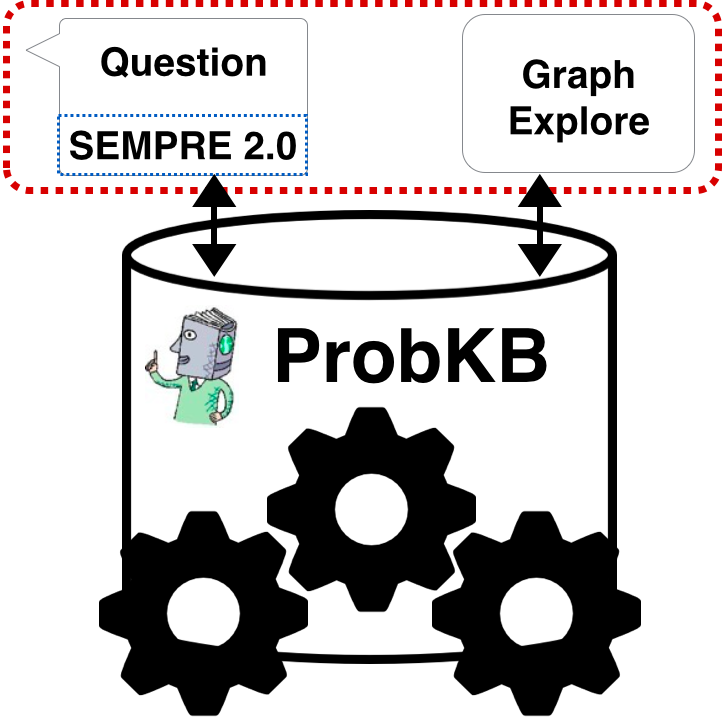
\includegraphics[width=\columnwidth,clip=true,trim=0cm 4cm 0cm 10cm]{images/qaarchitecture.png}
\centering
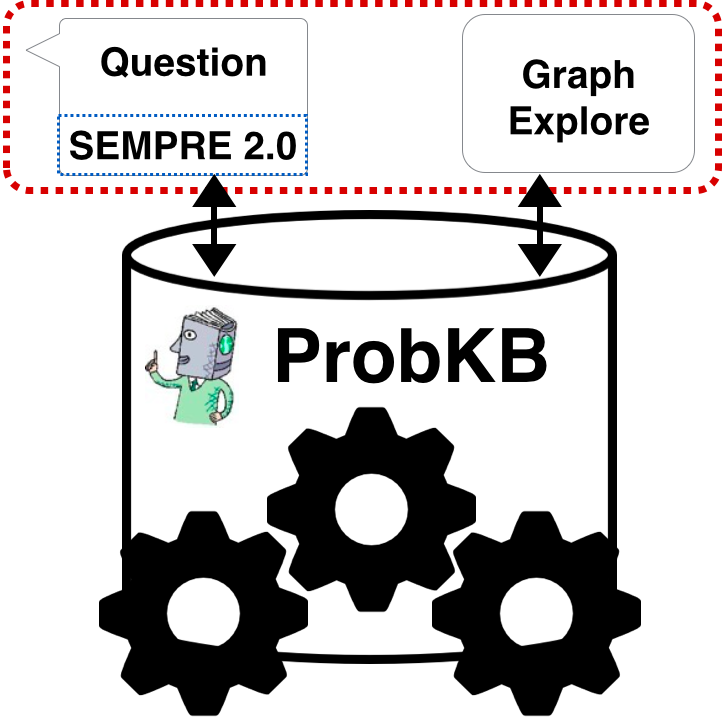
\includegraphics[width=0.6\columnwidth]{images/probqa-architecture.png}
\caption{Question answering system architecture.}
\label{fig:qaarchitecture}
\end{figure}

